\documentclass[tikz,border=2pt]{standalone}
\usepackage{xcolor}
\begin{document}
% III*_-1
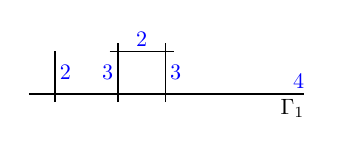
\begin{tikzpicture}[xscale=1,yscale=0.9]
\draw[thick,shorten >=2] (-1/3,0)--(97/30,0) node[inner sep=2pt,blue,above left,scale=0.8] {4} node[inner sep=2pt,below left,scale=0.8] {$\Gamma_1$};
\draw[shorten <=-3pt] (0,0)--node[inner sep=2pt,scale=0.8,blue,right] {2} (0,3/5);
\draw[shorten <=-3pt, shorten >=-3pt] (4/5,0)--node[inner sep=2pt,scale=0.8,blue,left] {3} (4/5,3/5);
\draw[shorten <=-3pt, shorten >=-3pt] (4/5,3/5)--node[inner sep=2pt,scale=0.8,blue,above] {2} (7/5,3/5);
\draw[shorten <=-3pt, shorten >=-3pt] (7/5,0)--node[inner sep=2pt,scale=0.8,blue,right] {3} (7/5,3/5);
\end{tikzpicture}
\end{document}
